\documentclass[tikz,border=3mm,multi=tikzpicture]{standalone}
\usepackage[utf8]{inputenc}
\usepackage[T1]{fontenc}
\usepackage{helvet}
\renewcommand{\familydefault}{\sfdefault}
\usepackage{tikz}
\usetikzlibrary{angles,quotes,calc,intersections}
\begin{document}

\tikzset{every node/.append style={font=\sffamily\small}}
% TikZ 1
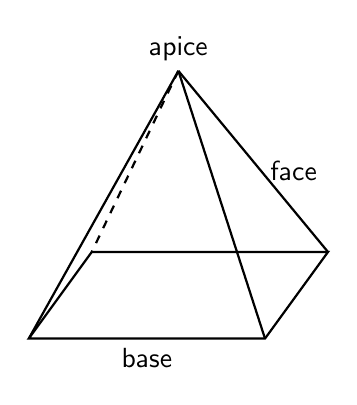
\begin{tikzpicture}[scale=1]
\coordinate (A) at (0,0); \coordinate (B) at (3,0); \coordinate (C) at (3.8,1.1); \coordinate (D) at (.8,1.1); \coordinate (V) at (1.9,3.4);
\draw[thick] (A)--(B)--(C)--(D)--cycle;
\draw[thick] (V)--(A); \draw[thick] (V)--(B); \draw[thick] (V)--(C); \draw[thick,dashed] (V)--(D);
\node[above] at (V) {apice};
\node[below] at (1.5,0) {base};
\node[right] at ($(V)!0.55!(C)$) {face};
\end{tikzpicture}
% TikZ 2
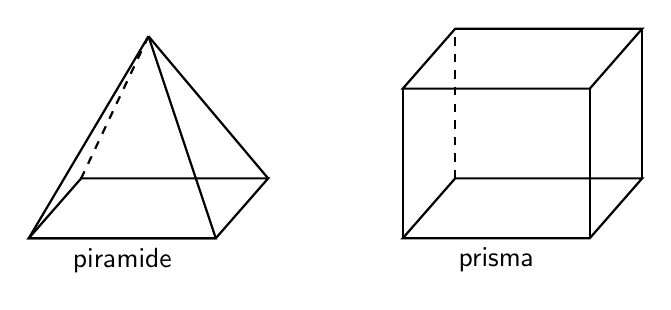
\begin{tikzpicture}[scale=.95]
\coordinate (A) at (0,0); \coordinate (B) at (2.5,0); \coordinate (C) at (3.2,.8); \coordinate (D) at (.7,.8); \coordinate (V) at (1.6,2.7);
\draw[thick] (A)--(B)--(C)--(D)--cycle; \draw[thick] (V)--(A)--(B)--(V); \draw[thick] (V)--(C); \draw[thick,dashed] (V)--(D);
\node[below] at (1.25,0) {piramide};
\coordinate (E) at (5,0); \coordinate (F) at (7.5,0); \coordinate (G) at (8.2,.8); \coordinate (H) at (5.7,.8);
\coordinate (I) at (5,2); \coordinate (J) at (7.5,2); \coordinate (K) at (8.2,2.8); \coordinate (L) at (5.7,2.8);
\draw[thick] (E)--(F)--(G)--(H)--cycle; \draw[thick] (I)--(J)--(K)--(L)--cycle;
\draw[thick] (E)--(I); \draw[thick] (F)--(J); \draw[thick] (G)--(K); \draw[thick,dashed] (H)--(L);
\node[below] at (6.25,0) {prisma};
\end{tikzpicture}


% TikZ 3
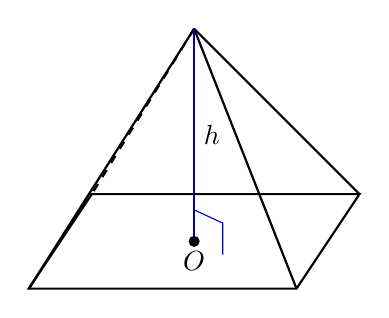
\begin{tikzpicture}[scale=1]
\coordinate (A) at (0,0); \coordinate (B) at (3.4,0); \coordinate (C) at (4.2,1.2); \coordinate (D) at (.8,1.2); \coordinate (O) at (2.1,.6); \coordinate (V) at (2.1,3.3);
\draw[thick] (A)--(B)--(C)--(D)--cycle;
\draw[thick] (V)--(A); \draw[thick] (V)--(B); \draw[thick] (V)--(C); \draw[thick,dashed] (V)--(D);
\draw[blue!70!black,thick] (V)--(O);
\pic[draw=blue!70!black, angle radius=4mm] {right angle=V--O--B};
\fill (O) circle (2pt);
\node[right] at ($(V)!0.5!(O)$) {$h$};
\node[below] at (O) {$O$};
\end{tikzpicture}
% TikZ 4
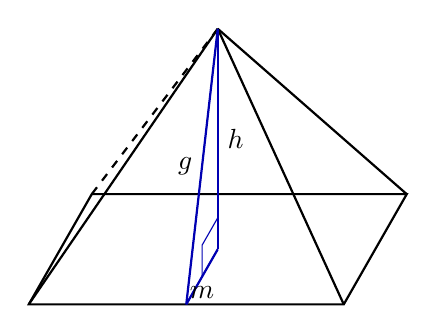
\begin{tikzpicture}[scale=1]
\coordinate (A) at (0,0); \coordinate (B) at (4,0); \coordinate (C) at (4.8,1.4); \coordinate (D) at (.8,1.4); \coordinate (O) at (2.4,.7); \coordinate (M) at (2,0); \coordinate (V) at (2.4,3.5);
\draw[thick] (A)--(B)--(C)--(D)--cycle;
\draw[thick] (V)--(A); \draw[thick] (V)--(B); \draw[thick] (V)--(C); \draw[thick,dashed] (V)--(D);
\draw[blue!70!black,thick] (V)--(O);
\draw[blue!70!black,thick] (O)--(M);
\draw[blue!70!black,thick] (V)--(M);
\pic[draw=blue!70!black, angle radius=4mm] {right angle=V--O--M};
\node[right] at ($(V)!0.5!(O)$) {$h$};
\node[below] at ($(O)!0.5!(M)$) {$m$};
\node[left] at ($(V)!0.5!(M)$) {$g$};
\end{tikzpicture}


% TikZ 5
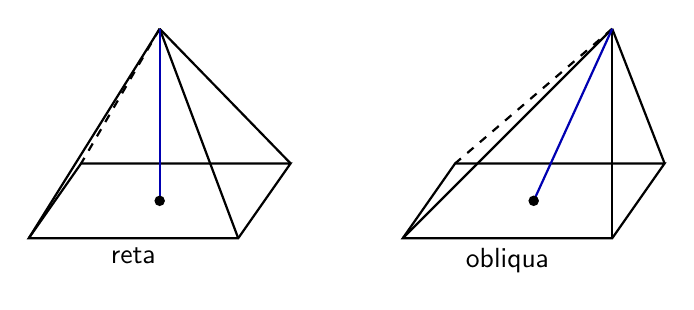
\begin{tikzpicture}[scale=.95]
\coordinate (A) at (0,0); \coordinate (B) at (2.8,0); \coordinate (C) at (3.5,1); \coordinate (D) at (.7,1); \coordinate (O) at (1.75,.5); \coordinate (V) at (1.75,2.8);
\draw[thick] (A)--(B)--(C)--(D)--cycle; \draw[thick] (V)--(A); \draw[thick] (V)--(B); \draw[thick] (V)--(C); \draw[thick,dashed] (V)--(D);
\draw[blue!70!black,thick] (V)--(O); \fill (O) circle (2pt);
\node[below] at (1.4,0) {reta};
\coordinate (E) at (5,0); \coordinate (F) at (7.8,0); \coordinate (G) at (8.5,1); \coordinate (H) at (5.7,1); \coordinate (P) at (6.75,.5); \coordinate (W) at (7.8,2.8);
\draw[thick] (E)--(F)--(G)--(H)--cycle; \draw[thick] (W)--(E); \draw[thick] (W)--(F); \draw[thick] (W)--(G); \draw[thick,dashed] (W)--(H);
\draw[blue!70!black,thick] (W)--(P); \fill (P) circle (2pt);
\node[below] at (6.4,0) {obliqua};
\end{tikzpicture}
% TikZ 6
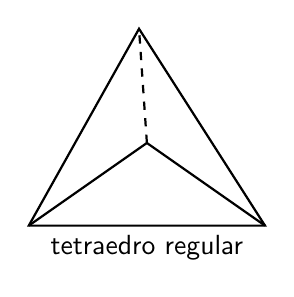
\begin{tikzpicture}[scale=1]
\coordinate (A) at (0,0); \coordinate (B) at (3,0); \coordinate (C) at (1.4,2.5); \coordinate (D) at (1.5,1.05);
\draw[thick] (A)--(B)--(C)--cycle;
\draw[thick] (D)--(A); \draw[thick] (D)--(B); \draw[thick,dashed] (D)--(C);
\node[below] at (1.5,0) {tetraedro regular};
\end{tikzpicture}
\end{document}
